\pdfoutput=1
\documentclass[10pt]{beamer}

%STANDARD PREAMBLE
%https://tex.stackexchange.com/questions/68821/is-it-possible-to-create-a-latex-preamble-header
\usepackage{../../rsrc/beamer_preamble}

%% ALLOW FOR ITEMIZE ENVIRONMENTS WITH NO PRECEDING
% SPACING, IF DESIRED
% Reference: https://tex.stackexchange.com/questions/86054/how-to-remove-the-whitespace-before-itemize-enumerate
%\usepackage{enumitem}% http://ctan.org/pkg/enumitem 
\usepackage{paralist}

% RANDOM VARIABLE
\newcommand{\x}{X}
\newcommand{\y}{Y}

%SUMS
\newcommand{\sumn}{\sum_{i=1}^{n}}


% ASSIGNMENTS
\newcommand{\assign}{z} %hardassignments
\newcommand{\Assign}{Z}
\newcommand{\soft}{r} %soft assignments

%%%% SUPPORT MAKING \subsectionpage
\AtBeginSection{\frame{\sectionpage}}
\AtBeginSubsection{\frame{\subsectionpage}}

\title{Expectation Maximization}

\begin{document}

\maketitle
\begin{frame}{Table of contents}
  \setbeamertemplate{section in toc}[sections numbered]
  \setbeamertemplate{subsection in toc}[subsections numbered]
   \setbeamertemplate{subsection in toc}{\leavevmode\leftskip=3.2em\rlap{\hskip-2em\inserttocsectionnumber.\inserttocsubsectionnumber}\inserttocsubsection\par} %indents the subsections
  \tableofcontents
\end{frame}

\begin{frame}{Acknowledgements}
This slide deck borrows heavily from an excellent course on statistical ML by Peter Orbanz.  
\vfill
Another important resource was Christopher Bishop's Machine Learning textbook.
\end{frame}

\section{The k-means algorithm}

\begin{frame}{Clustering}
\begin{sblock}{Problem}
\begin{minipage}{0.6\textwidth}
\begin{itemize}
\item Given: Data $x_1, ..., x_n$.
\item Assumption: Each data point belongs to exactly one group or class. These groups are called \bf{clusters}.
\item Our task is to find the clusters, given only the data.
\end{itemize}
\end{minipage} 
\hfill
\begin{minipage}{0.3\textwidth}
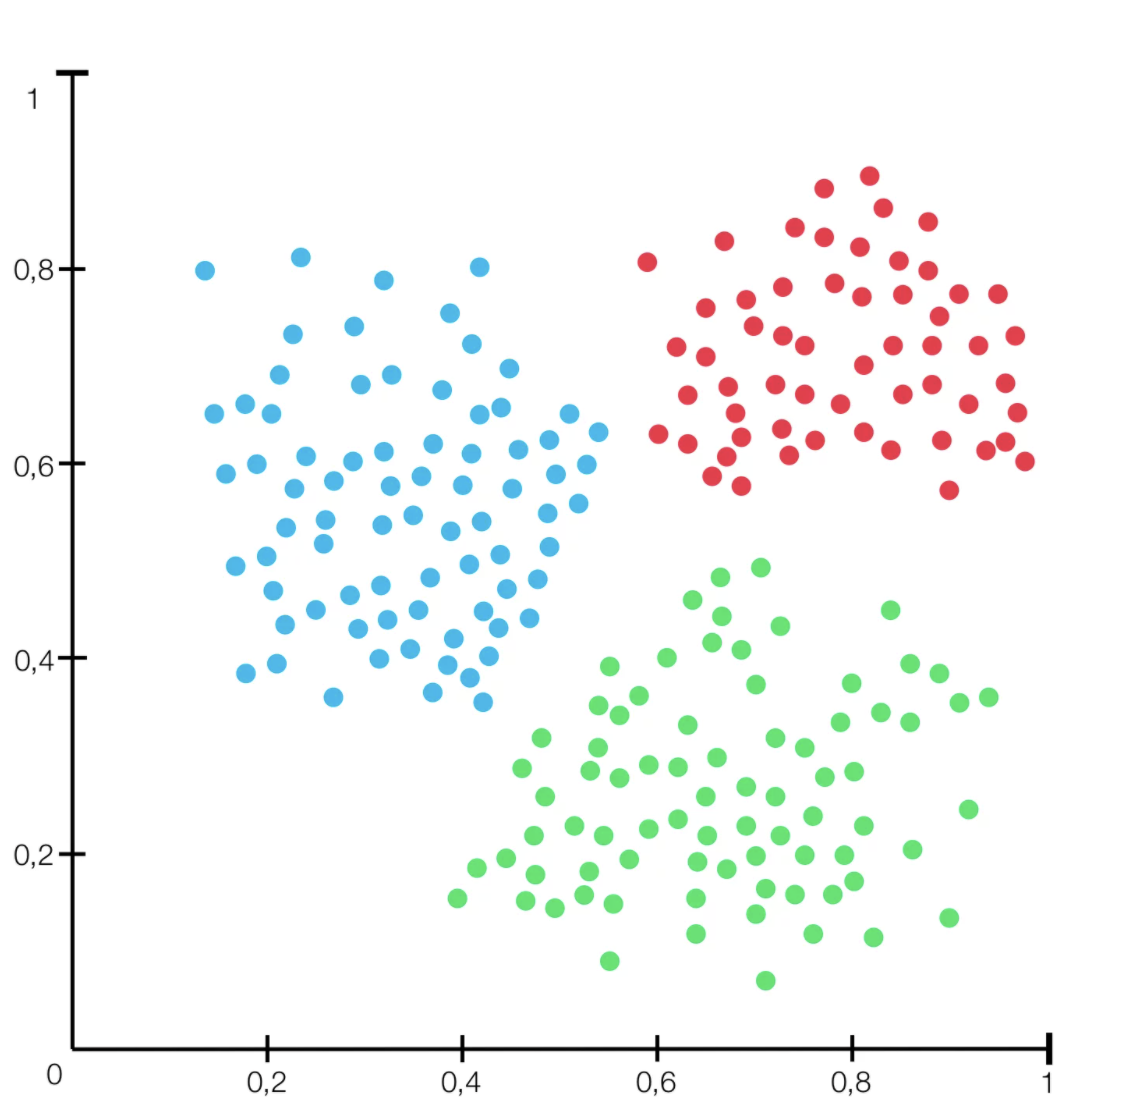
\includegraphics[width=\textwidth]{images/clustering}
\end{minipage} 

\end{sblock}

\begin{sblock}{Representation}
Fror $K$ clusters, we encode assignments to clusters as a vector $\+\assign \in \set{1,...,K}^n$ where:
\[ \+\assign_i = k \iff x_i \text{ assigned to cluster } k \]
\end{sblock}

%\begin{sblock}{Clustering and classification}
%Clustering is the ``unsupervised" counterpart to classification.   There is no training data and no labels, only one, unlabeled data set. 
%\end{sblock}

\end{frame}



%\begin{frame}{Example: Image Segmentation}
%\scriptsize
%\begin{sblock}{Image Segmentation}
%\bf{Image segmentation} is the problem of partitioning an image into ``coherent" regions.  The problem is not well-posed: Its solution depends on the meaning of ``coherent".
%\end{sblock}
%
%\begin{sblock}{Example}
%\includegraphics[width=\textwidth]{images/image_segmentation}
%\end{sblock}
%
%\begin{sblock}{Segmentation as a clustering problem}
%\begin{itemize}
%\item For each pixel, place a small window around the pixel.  Extract features (measurements) from this window.  For the $i$-th pixel, represent measurements by a vector $x_i$.
%\item Compute a clustering of the data $x_1, ..., x_n$ with K clusters.
%\item Each cluster represents one segment.  In the images above, one cluster is colored blue, one green, one red.
%\end{itemize}
%
%\end{sblock}

%\end{frame}


\begin{frame}{A very simple clustering algorithm: K-means}
\scriptsize
\begin{sblock}{K-means algorithm}
\begin{itemize}

\item Randomly choose K ``cluster centers" (the ``means") $\mu_1^{(0)}, ..., \mu_K^{(0)} \in \R^d$
\item Iterate until convergence ($j$ = iteration number):
	\begin{enumerate}
	\scriptsize
	\item Assign each $x_i$ to the closest (in Euclidean distance) mean:
	\[ \assign_i^{(j+1)} := \arg\min_{k \in \set{1,...,K}} ||x_i - \mu_k^{(j)} || \]
	\item Recompute each $\mu_k^{(j)}$ as the mean of all points assigned to it.
	\[ \mu_k^{(j+1)} := \df{1}{|i : \assign_i^{(j+1)} = k |}  \ds\sum_{i : \assign_i^{(j+1)} = k} x_i\]
	\end{enumerate}
\end{itemize}

\end{sblock}

\begin{sblock}{Convergence Criterion}
For example: Terminate when the total change of the means satisfies:
\[  \ds\sum_{k=1}^K || \mu_k^{(j+1)} - \mu_k^{(j)} || < \tau \]
The threshold value $\tau$ is set by the user.
\end{sblock}

\end{frame}

\begin{frame}{Illustration}
\begin{center}
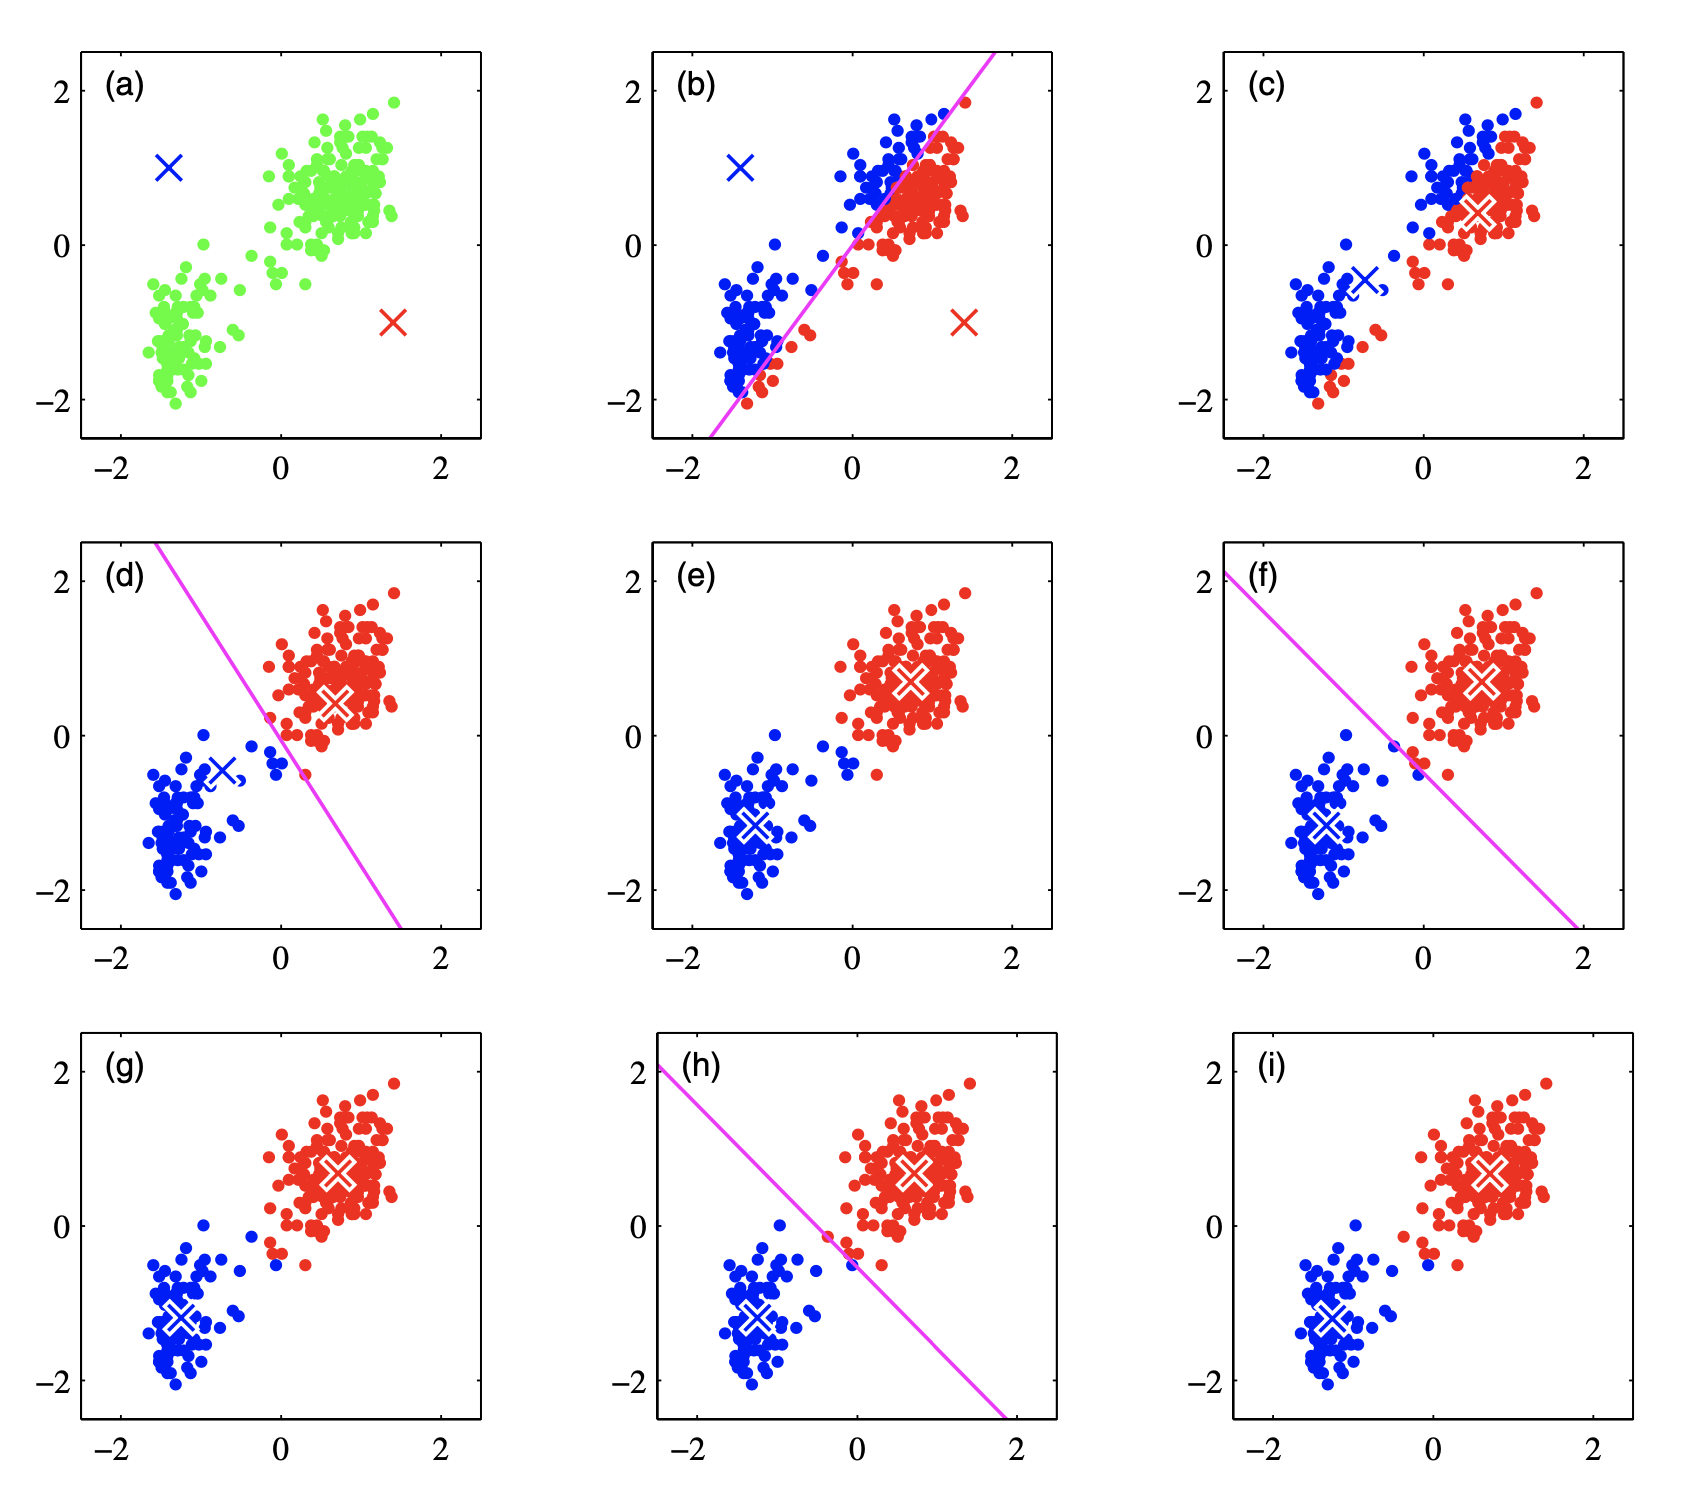
\includegraphics[width=.7\textwidth]{images/k_means}
\end{center}
\scriptsize Illustration of the  $K$-means algorithm using the re-scaled Old Faithful dataset (in green).  The initial choices for centers $\mu_1$ and $\mu_2$ are shown by the red and blue crosses, respectively.
\vfill
\hfill \tiny Image Credit: Christopher Bishop \\
\tiny \bf{Q:}  Look at this for a minute, who wants to try to walk us through what's happening?
\end{frame}


\begin{frame}{Application: Image Segmentation and Clustering}

\scriptsize 

\begin{sblock}{Image Segmentation}
 \bf{Image segmentation} is the problem of partitioning an image into ``coherent" regions.   The problem is not well-posed: Its solution depends on the meaning of ``coherent".
\end{sblock}

\begin{sblock}{$K$-means on images}
\begin{itemize}
\item Each pixel is treated as a separate point representing $\{R,G,B\}$ intensities.
\item Note: not sophisticated; spatial proximity ignored.
\end{itemize} 

\begin{center}
\begin{tikzpicture}
  % Put a picture at a tikz node. 
  %I'm not sure what the anchor does, exactly.
    \node[anchor=south west,inner sep=0] (image) at (0,0) {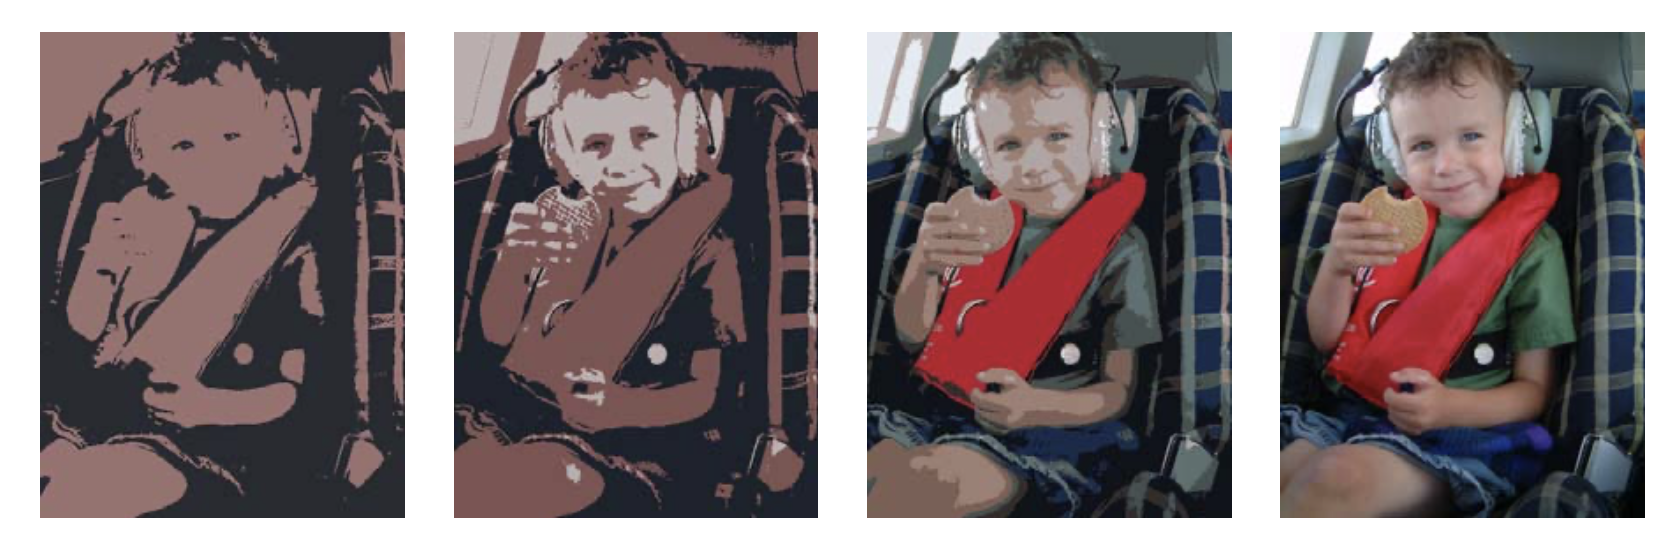
\includegraphics[width=.5\textwidth]{images/k_means_images}};
    % The scope environment induces relative coordinates to the picture.
    \begin{scope}[x={(image.south east)},y={(image.north west)}]
        \node[text=black, text width=2cm] at (.20, 1.2) {$K=2$};
        \node[text=black, text width=2cm] at (.45, 1.2) {$K=3$};
         \node[text=black, text width=2cm] at (.70, 1.2) {$K=10$};
        \node[text=black, text width=2cm] at (.95, 1.2) {original};
    \end{scope}
\end{tikzpicture}
\end{center}
\hfill \tiny Image Credit: Christopher Bishop \scriptsize

\end{sblock}
%\begin{itemize}
%\item Each pixel treated as a separate point representing $\{R,G,B\}$ intensities.
%\item \bf{Image segmentation} is the problem of partitioning an image into ``coherent" regions.    \tiny ($K$-means not sophisticated; spatial proximity ignored.) \scriptsize
%\item (Lossy) \bf{image compression} obtained by storing only the cluster identity $k$ and the \it{code-book vectors} $\+\mu_k$.
%\end{itemize}



\begin{sblock}{Utility for image compression}
\it{(Lossy) image compression} is a side effect; one can store only the cluster identity $k$ and the \it{code-book vectors} $\+\mu_k$.
\end{sblock}
%\begin{itemize}
%\item For each pixel, place a small window around the pixel.  Extract features (measurements) from this window.  For the $i$-th pixel, represent measurements by a vector $x_i$.
%\item Compute a clustering of the data $x_1, ..., x_n$ with K clusters.
%\item Each cluster represents one segment.  In the images above, one cluster is colored blue, one green, one red.
%\end{itemize}

\end{frame}


\begin{frame}{Application: Anomaly Detection in Cybersecurity}

\begin{itemize}
\item Malware not uncommonly contains icons which look like legitimate applications (to try to trick the user into clicking on it.
\item Often these icons have slight blurriness, or color shifting, to avoid detection. 
\item Clustering algorithms (such as k-means,  t-SNE or HDBScan) can be used to identify if there is an embedded icon, what it is, and if it looks anomalous.
\end{itemize}
\begin{center}
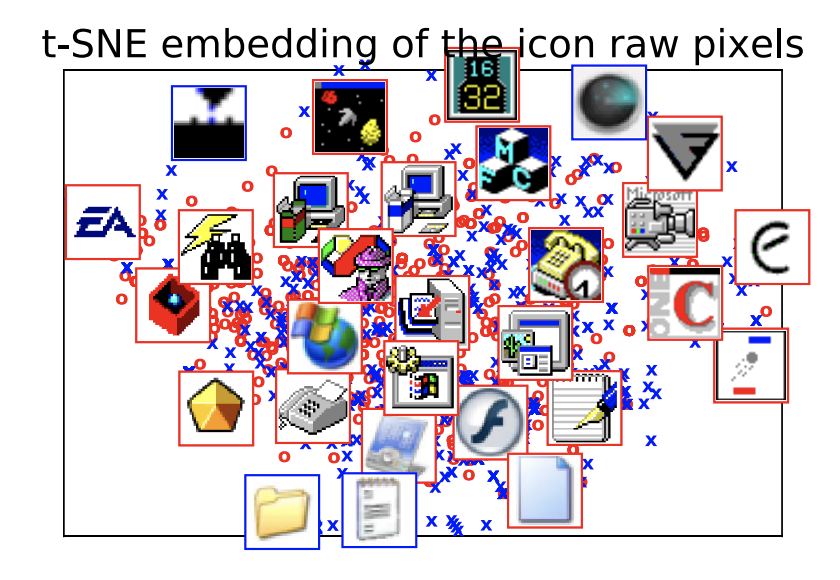
\includegraphics[width=.5\textwidth]{images/malware_icons}
\end{center}

\end{frame}

\begin{frame}{Python Demo}
\begin{center}
\href{https://github.com/JWarmenhoven/Coursera-Machine-Learning/blob/master/notebooks/Programming\%20Exercise\%207\%20-\%20K-means\%20Clustering\%20and\%20Principal\%20Component\%20Analysis.ipynb}{K-means demo in python}
\end{center}
\end{frame}


\begin{frame}{$K$-Means: Gaussian Interpretation}
	\scriptsize
\begin{sblock}{$K$ Gaussians}
Consider the following algorithm:
\begin{itemize}
\item Suppose each $\mu_k$ is the expected value of a Gaussian density $p(x|\mu_k, \mathbb{I})$ with unit covariance.  
\item Start with $K$ randomly chosen means and iterate.
	\begin{enumerate}
	\scriptsize
	\item Assign each $x_i$ to the Gaussian under which it has the highest density.
	\item Given the assignments, fit $p(x|\mu_k, \mathbb{I})$ by maximum likelihood estimation of $\mu_k$ from all points assigned to cluster $k$.
	\end{enumerate}
\end{itemize}
\end{sblock}

\begin{sblock}{Comparison to $K$-means}
\begin{itemize}
	\scriptsize
\item Since the Gaussians are spherical with identity covariance, the density $p(x|\mu_k, \mathbb{I})$  is largest for the mean $\mu_j$ which is closest to $x_i$ in Euclidean distance.  \tiny (Why?) \scriptsize
\item The maximum likelihood estimator of $\mu_k$ is 
	\[ \mu_k^{(j+1)} := \df{1}{|i : \assign_i^{(j+1)} = k |}  \ds\sum_{i : \assign_i^{(j+1)} = k} x_i\]
	This is precisely the $K$-means algorithm!
\end{itemize}

\end{sblock}
\end{frame}

\begin{frame}{What next}
\begin{itemize}
\item We will discuss a more sophisticated version of $K$-means called the \it{Expectation-Maximization (EM) algorithm.}

\item EM gives
	\begin{enumerate}
	\item A better statistical explanation of what is going on. 
	\item A direct generalization to other distributions.  We can consider Gaussians with general covariance structure, or other distributions as well.
    \item Better support for the anomaly detection use case.
	\end{enumerate}
\end{itemize}

\end{frame}

\section{Mixture Models} 

\begin{frame}{Finite mixture models}


\begin{sblock}{Finite Mixture Model}
A finite mixture model is a distribution with density of the form
\[ \pi(x) = \ds\sum_{k=1}^K c_k \; p(x \cond \theta_k) \]
where $\sum_k c_k =1$ and $c_k \geq 0$.

\end{sblock}
\begin{sblock}{Example: Finite mixture of Gaussians}
\begin{center}
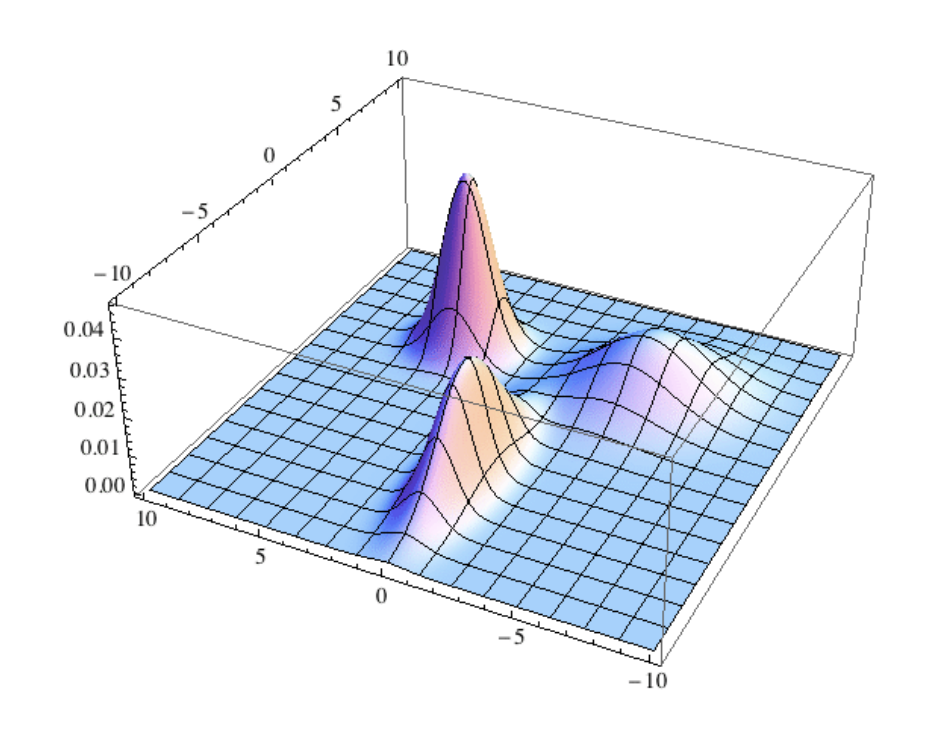
\includegraphics[width=.5\textwidth]{images/gmm}
\end{center}

\end{sblock}

\end{frame}

% GMM for anomaly detection

\begin{frame}{Illustration}
\begin{sblock}{Mixture of two Gaussians}
\begin{minipage}{0.4\textwidth}
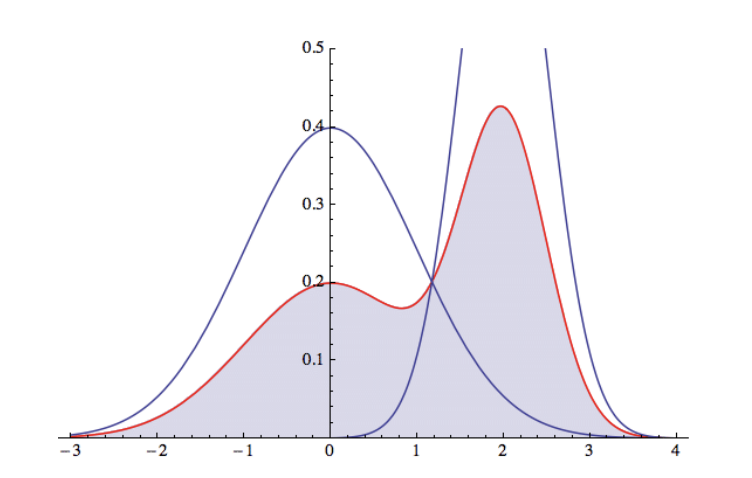
\includegraphics[width=\textwidth]{images/gmm_weights_1}
\end{minipage} 
\hfill 
\begin{minipage}{0.5\textwidth}
The curve outlined in red is the mixture
\[ \pi(x) = 0.5 \, p(x \cond 0, 1) + 0.5 \, p(x \cond 2, 0.5) \]
where $p$ is the Gaussian density.  The blue curves are the component densities.
\end{minipage} 

\end{sblock}
\vfill

\begin{sblock}{Influence of the weights}
\begin{minipage}{0.4\textwidth}
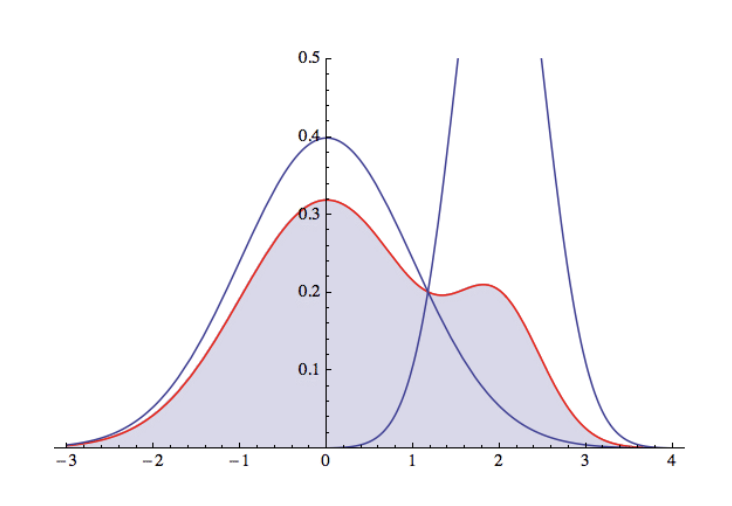
\includegraphics[width=\textwidth]{images/gmm_weights_2}
\end{minipage} 
\hfill 
\begin{minipage}{0.5\textwidth}
Here, the weights $c_1=c_2 =0.5$ above have been changes to $c_1 = 0.8$ and $c_2 = 0.2$.  The component distributions are the same as above. 
\end{minipage} 

\end{sblock}
\end{frame}

\begin{frame}{Sampling}
\scriptsize

\begin{sblock}{Sampling from a finite mixture}
For a finite mixture with fixed parameters $c_k$ and $\theta_k$, the two-step sampling procedure is:
\begin{enumerate}
\item Choose a mixture component at random. Each component $k$ is selected with probability $c_k$.
\item Sample $x_i$ from $p(x|\theta_k)$.
\end{enumerate}
\bf{Note}: We always repeat both steps, i.e. for $x_{i+1}$, we choose again choose a (possibly different) component at random.

\end{sblock}
\tiny \hfill Note that k-means does not support sampling new points.


\begin{center}
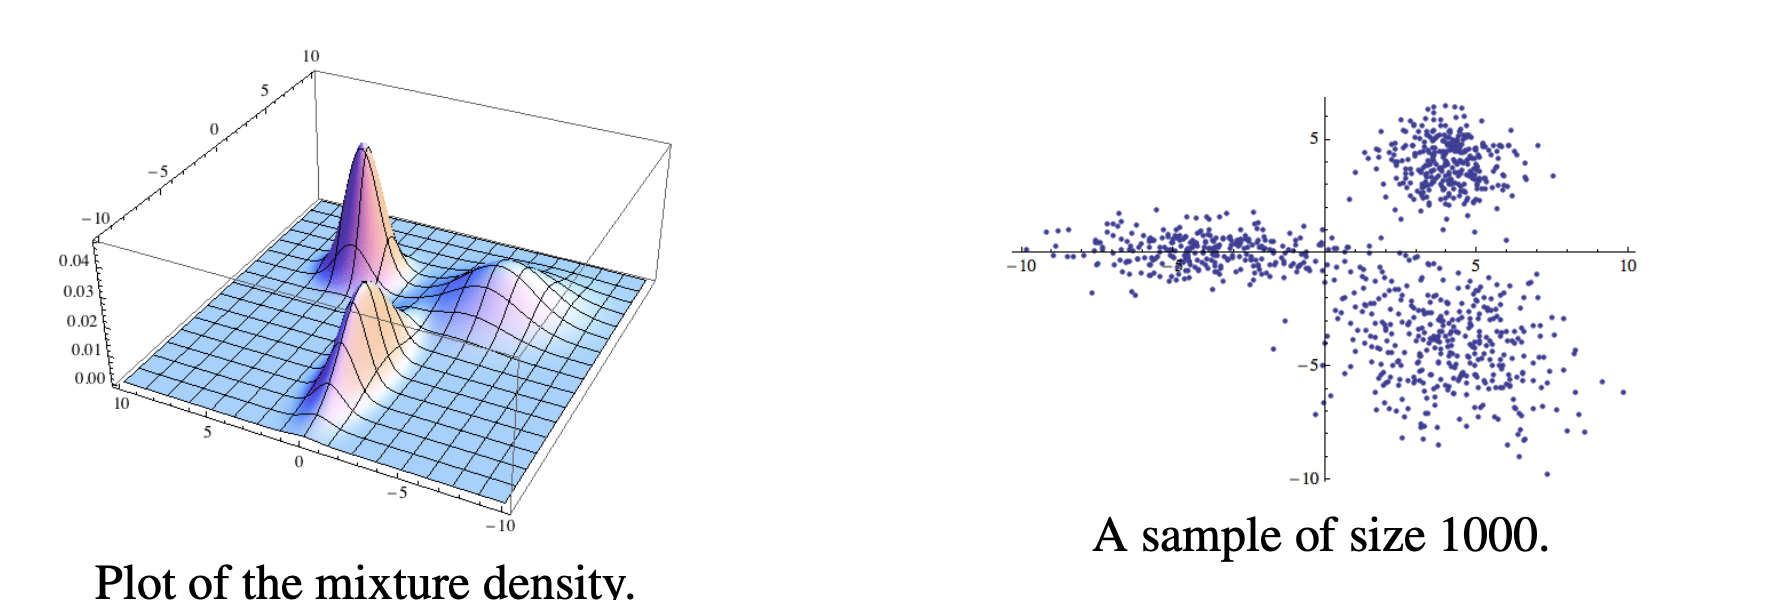
\includegraphics[width=\textwidth]{images/gmm_sampling}
\end{center} 


\end{frame}

\begin{frame}{Mixture estimation}
\footnotesize
\begin{sblock}{Maximum likelihood for finite mixtures}
Writing down the maximum likelihood problem is straightforward:
\[ (\widehat{\+c}, \widehat{\+\theta}) = (\widehat{c}_1, ..., \widehat{c}_K, \widehat{\theta}_1, ..., \widehat{\theta}_K) = \arg\max_{\+c, \+\theta} \ds\prod_{i=1}^n  \bp{ \ds\sum_{k=1}^K c_k \, p(x_1 | \theta_k)} \]

The maximality equation for the logarithmic likelihood is
\[ \df{\delta}{\delta (\+c, \+\theta) } \ds\sum_{i=1}^n \log \bp{ \ds\sum_{k=1}^K c_k \, p(x_1 | \theta_k)}  = 0 \] 
The component equation for each $\theta_k$ is:
\[ \ds\sum_{i=1}^n \df{c_k \frac{\delta}{\delta \theta_k} p(x_i|\theta_k)}{\sum_{k=1}^K c_k p(x_i|\theta_k)}  =0 \] 
Solving this problem is analytically infeasible (note that we cannot multiply out the
denominator, because of the sum over $i$). Even numerical solution is often difficult.
\end{sblock}

\end{frame}

\begin{frame}{Latent Variables}


\begin{sblock}{Cluster assignments}
\begin{itemize}
\item The mixture assumption implies that each $x_i$ was generated from one component.
\item For each $x_i$, we again use an \bf{assignment variable} $\assign_i \in \set{1,...,K}$ which encodes which cluster $x_i$ was sampled from.
\end{itemize}
\end{sblock}

% https://tex.stackexchange.com/questions/300098/draw-a-node-as-a-square-with-tikz
\begin{minipage}{.45\textwidth}
  \centering
  \scalebox{0.7}{
  \tikz[square/.style={regular polygon,regular polygon sides=4}]{ %
     \node[square, draw](pi){$\pi$}; %
     \node[latent, below = of pi](xi){$x_i$};
     \edge{pi}{xi}
      \plate[inner sep=0.25cm, xshift=0cm, yshift=0cm] {plate1} {(xi)} {$N$}; %
  }
 }
\end{minipage} \hfill
\begin{minipage}{.10\textwidth}
\[ \Rightarrow \]
\end{minipage} \hfill
\begin{minipage}{.45\textwidth}
  \centering
  \scalebox{0.7}{
  \tikz[square/.style={regular polygon,regular polygon sides=4}]{ %
     \node[square, draw](c){$\+c$}; %
      \node[square, draw, right = of c](mu){$\+\theta$}; %
     \node[latent, below = of c](zi){$\assign_i$};
     \node[latent, below = of mu](xi){$x_i$};
     \edge{c}{zi}
      \edge{mu}{xi}
     \edge{zi}{xi}
      \plate[inner sep=0.25cm, xshift=0cm, yshift=0cm] {plate1} {(xi)(zi)} {$N$}; %
  }
 }
\end{minipage} \hfill


\begin{sblock}{Latent Variables}
Since we do not know which component each $x_i$ was generated by, the values of the assignment variables are \it{unobserved}. Such variables whose values are not observed are called \bf{latent variables} or \bf{hidden variables}.
\end{sblock}
\end{frame}

\begin{frame}{Estimation with latent variables}

\begin{sblock}{Latent variables as auxiliary information}
If we knew the correct assignments $\assign_i$, we could:
\begin{itemize}
\item Estimate each component distribution $p(x|\theta_k)$ separately, using only the data assigned to cluster $k$.
\item Estimate the cluster proportions $c_k$ as $\widehat{c}_k = \frac{\text{\# points in cluster} \, k}{n}$
\end{itemize}

\end{sblock}
\begin{sblock}{EM algorithm: Idea}
The EM algorithm estimates values of the latent variables to simplify the estimation problem. EM alternates between two steps:
\begin{enumerate}
\item Estimate assignments $\assign_i$  given current estimates of the parameters $c_k$ and $\theta_k$ ("E-step").
\item Estimate parameters $c_i$ and $\theta_k$ given current estimates of the assignments ("M-step").
\end{enumerate}

These two steps are iterated repeatedly.
\end{sblock}
\end{frame}


\begin{frame}{Representation of Assignments}
\footnotesize
We re-write the assignments as vectors of length $K$:

\[ \+x_i \, \text{in cluster } k \quad \text{as} \quad \Assign_i := 
\begin{bmatrix}
0  \\
\vdots  \\
0  \\
1 \\
0  \\
\vdots  \\
0 
\end{bmatrix} \leftarrow k\text{th entry}
 \]
 so $\Assign_{ik}=1$ if $x_i$ in cluster k, and $\Assign_{ik} =0$ otherwise. \\
 \vfill
 We collect the vectors into a matrix
 \[ 
 \+\Assign := 
\begin{bmatrix}
\Assign_{11} & ... &  \Assign_{1K}\\
\vdots & & \vdots \\
\Assign_{n1} & ... &  \Assign_{nK}\\
\end{bmatrix} \
 \]
Note: Rows = observations, columns = clusters \\
Row sums = 1, column sums = cluster sizes.
\end{frame}

\begin{frame}{E-Step}
\footnotesize
\begin{sblock}{Hard vs. soft assignments}
\begin{itemize}
\item The vectors $\Assign_i$ are ``hard assignments" with values in $\set{0,1}$ (as in $k$-means)
\item EM computes ``soft assignments" $\soft_{ik}$ with values in $[0,1]$.\footnote{\tiny Once the algorithm terminates, each point could still be assigned to a cluster by setting
\[ \assign_i = \arg\max_k \soft_{ik} \]}
\item The vectors $\Assign_i$ are the the latent variables in the EM algorithm.  The $\soft_{ik}$ are their current estimates
\end{itemize}
\end{sblock}

\begin{sblock}{Assignment probabilities}
The soft assignments are computed as
\[ \soft_{ik} = \df{c_k \, p(x_i \cond \theta_k)}{ \sum_{l=1}^K c_l  \, p(x_i \cond \theta_l)} \]
They can be interpreted as
\[  \soft_{ik} := \E [\Assign_{ik} \cond x_i, \+c, \+\theta] = \text{Pr} \set{x_i \text{ generated by component } k \cond \+c, \+\theta} \]
\end{sblock}
\end{frame}

\begin{frame}{M-Step (1)}

\begin{sblock}{Objective}
The M-step re-estimates $\+c$ and $\+\theta$.  In principle, we use maximum likelihood within each cluster, but we have to combine it with the use of weights $\soft_{ik}$ instead of $\Assign_{ik}$
\end{sblock}

\begin{sblock}{Cluster sizes}
If we knew which points belong to which cluster, we could estimate the cluster proportions $c_k$ by counting points:
\[ \widehat{c}_k = \df{\text{\# points in cluster } k}{n} = \df{\sum_{i=1}^n \Assign_{ik}}{n}\]
Since we do not know $\Assign_{ik}$, we substitute our current best guess, which is the expectations $\soft_{ik}$
\[ \widehat{c}_k  = \df{\sum_{i=1}^n \soft_{ik}}{n}\]
\end{sblock}
\end{frame}


\begin{frame}{M-Step (2)}
\footnotesize
\begin{sblock}{Gaussian special case}
The estimation of the component parameters $\theta$ depends on which distribution we choose for $p$.  For now, we assume a Gaussian. 
\end{sblock}
\begin{sblock}{Component parameters}
We use maximum likelihood to estimate $\theta=(\mu, \Sigma)$.  We can write the MLE of $\mu_k$ as 
\[ \widehat{\mu}_k =  \df{1}{\text{\# points in cluster } k}  \ds\sum_{i : x_i \, \text{in} \; k} x_i = \df{\sum_{i=1}^n  \Assign_{ik} x_i} {\sum_{i=1}^n \Assign_{ik}}\]
By substituting current best guesses $(=\soft_{ik})$ again, we get
\[ \widehat{\mu}_k = \df{\sum_{i=1}^n  \soft_{ik} x_i}{\sum_{i=1}^n \soft_{ik}}\]
For the covariance matrices:
\[ \widehat{\Sigma}_k = \df{ \sum_{i=1}^n \soft_{ik} (x_i - \widehat{\mu}_k ) (x_i - \widehat{\mu}_k )^T }{ \sum_{i=1}^n \soft_{ik}} \]
\end{sblock}
\end{frame}

\begin{frame}{Notation Summary}
\begin{sblock}{Assignment probabilities}
\[ 
 \+\soft := 
\begin{bmatrix}
\soft_{11} & ... & \soft_{1K}\\
\vdots & & \vdots \\
\soft_{n1} & ... &  \soft_{nK}\\
\end{bmatrix} 
= \E \bb{
\begin{bmatrix}
\Assign_{11} & ... & \Assign_{1K}\\
\vdots & & \vdots \\
\Assign_{n1} & ... &  \Assign_{nK}\\
\end{bmatrix} 
} =
\begin{bmatrix}
\E[\Assign_{11}] & ... & \E[\Assign_{1K}]\\
\vdots & & \vdots \\
\E[\Assign_{n1}] & ... &  \E[\Assign_{nK}]\\
\end{bmatrix} 
 \]
 
\end{sblock}
\begin{sblock}{Mixture parameters}
\[ \+\tau = (\+c, \+\theta), \quad \+c = \text{cluster proportions } \quad \+\theta = \text{component parameters} \]
\end{sblock}
\begin{sblock}{Iterations}
$\+\theta^{(j)}, \+\soft^{(j)}, ...$ = values in $j$th iteration 
\end{sblock}
\end{frame}

\begin{frame}{Summary: EM for Gaussian Mixture}
\footnotesize
\begin{sblock}{Gaussian special case}
\[  \theta = (\mu, \Sigma) \, \text(mean \, \& \, covariance) \quad p(x \cond \theta) = p(x \cond \mu, \Sigma) \, \text{(Gaussian density)}\]
\end{sblock}
\begin{sblock}{Algorithm}
The EM algorithm for a finite mixture of Gaussians looks like this
\begin{enumerate}
\item \bf{Initialize:} Choose (e.g., random) values $c_k^{(0)}$ and $\theta_k^{(0)}$.
\item \bf{E-Step:} Recompute the assignment weight matrix as
\[ \soft_{ik}^{(j+1)} = \df{c_k^{(j)} p(x_i \cond \theta_k^{(j)})}{ \sum_{l=1}^K c_l^{(j)} p(x_i \cond \theta_l^{(j)})}\]
\item \bf{M-Step:} Recompute the proportions $c_k$ and parameters  $\theta=(\mu, \Sigma)$ as


\[ \mu_k^{(j+1)} = \df{\sumn \soft_{ik}^{(j+1)} x_i}{ \sumn \soft_{ik}^{(j+1)}} \quad \text{and} \quad \Sigma_k^{(j+1)}= \df{ \sumn \soft_{ik}^{(j+1)}   (x_i  -\mu_k^{(j+1})  (x_i  -\mu_k^{(j+1)})^T}{ \sumn \soft_{ik}^{(j+1)}}   \] 
\end{enumerate}
The E-Step and M-Step are repeated alternatingly until convergence criterion (e.g. threshold) is satisfied.
\end{sblock}
\end{frame}

\begin{frame}{EM: Illustration}

\begin{sblock}{EM for a mixture of two Gaussians}
\begin{center}
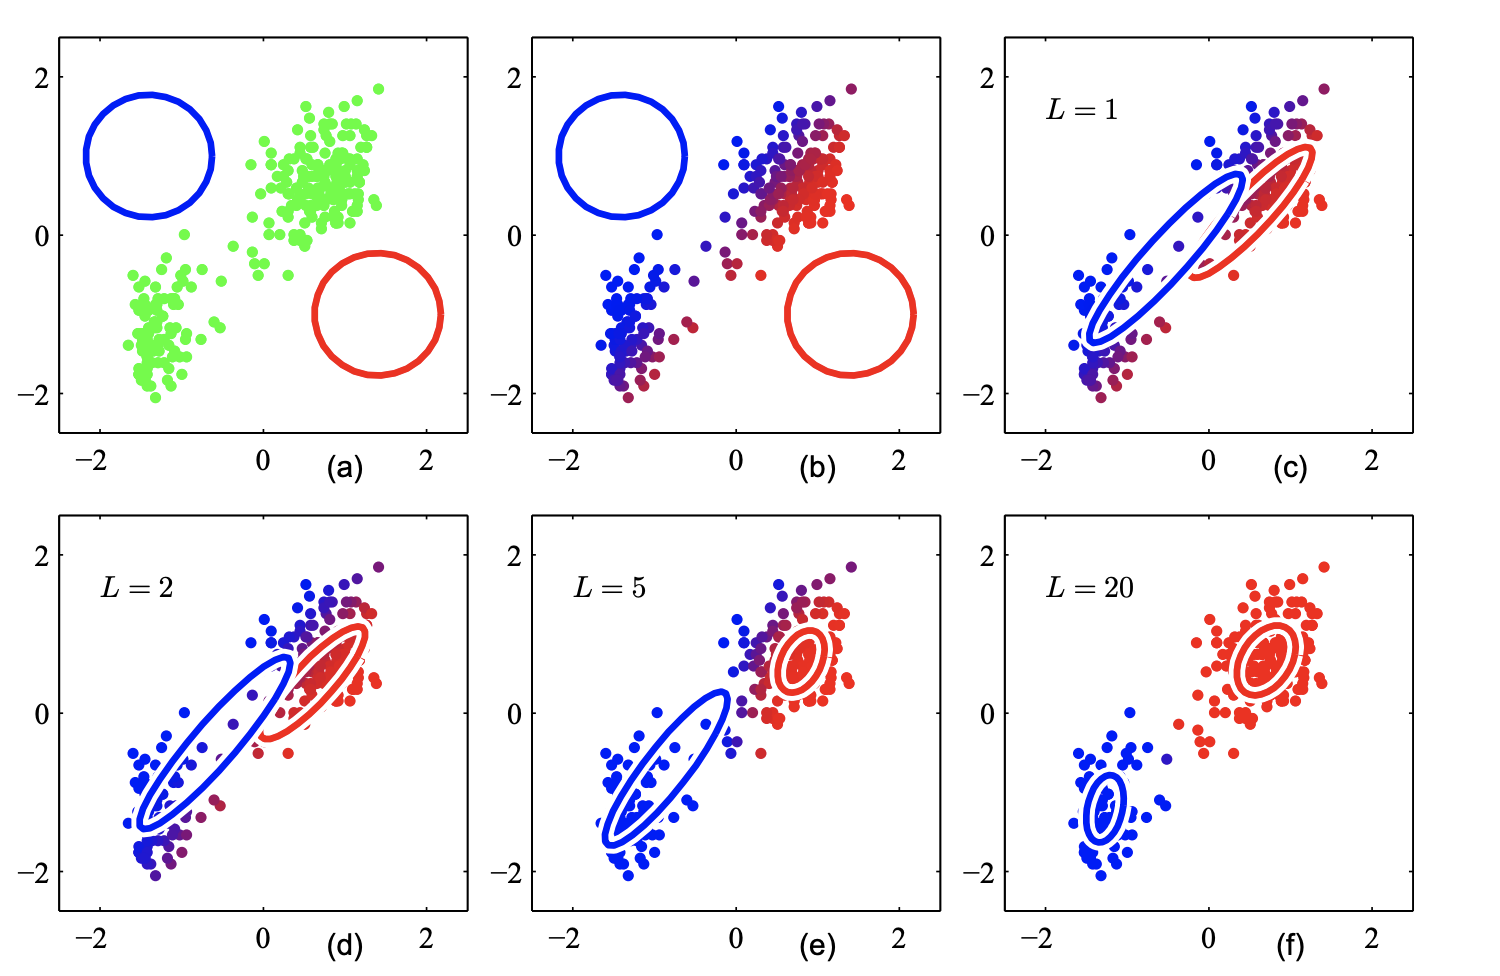
\includegraphics[width=.6\textwidth]{images/em_for_mixture_of_two_gaussians}
\end{center}

\end{sblock}

The algorithm fits both the mean and the covariance parameter.
\end{frame}


\begin{frame}{Two group activities}
\begin{enumerate}
\item Implementational
\item API Usage / Conceptual
\end{enumerate}

\end{frame}


\begin{frame}{GMMs as Universal Approximators}

\begin{quote}
A Gaussian mixture model is a universal approximator of densities, in the sense that any smooth density can be approximated with any specific nonzero amount of error by a Gaussian mixture model with enough components.
\end{quote}

\hfill \tiny Ian Goodfellow et al. 2016
\vfill
\tiny More formally, if $\mathcal{P}(\R^d)$  is the set of probability Borel measures on $\R^d$ (with its Euclidean topology), then ``Gaussian mixtures" (a.k.a. convex combinations of Gaussian measures) are dense in $\mathcal{P}(\R^d)$ for the  weak*  topology.
\vfill \vfill \vfill
\tiny \bf{Q:} So why not use GMM's for everything?

\end{frame}
% A's: Known support,  computation efficiency / estimation power (e.g. in high dimensions)

\begin{frame}{Other Mixture Models}
The mixture components do not need to be Gaussian in order for the model to be well-posed, and for EM to estimate the parameters.   \\
\vfill 
\begin{sblock}{Example: mixture of two betas}
\begin{center}
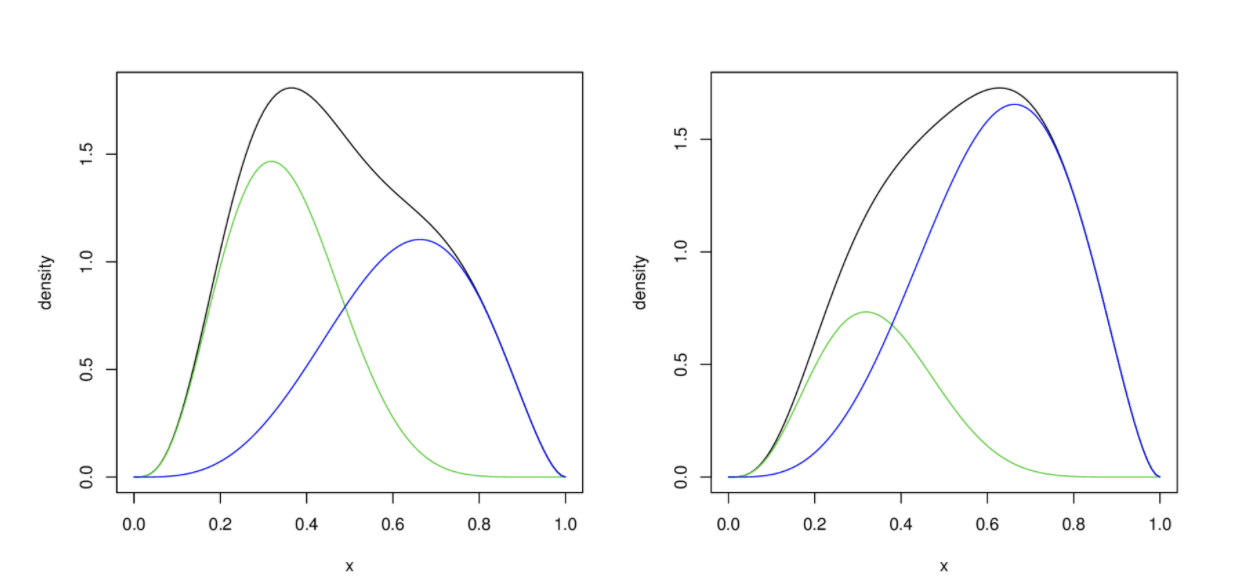
\includegraphics[width=.6\textwidth]{images/mixture_of_betas}

\end{center}
\scriptsize Shown are two beta mixture models, each with two components.  The models have fixed components but differ in their mixture weights: $\+c = (.25, .75)$ vs. $\+c = (.75, .25)$.
\end{sblock}

\vfill \vfill \vfill
\tiny \textbf{Q:} Under what conditions might one use a mixture of betas rather than a mixture of Gaussians?
\end{frame}

\begin{frame}{Other Mixture Models}

\begin{sblock}{Example: mixture of two Gammas}
\begin{center}
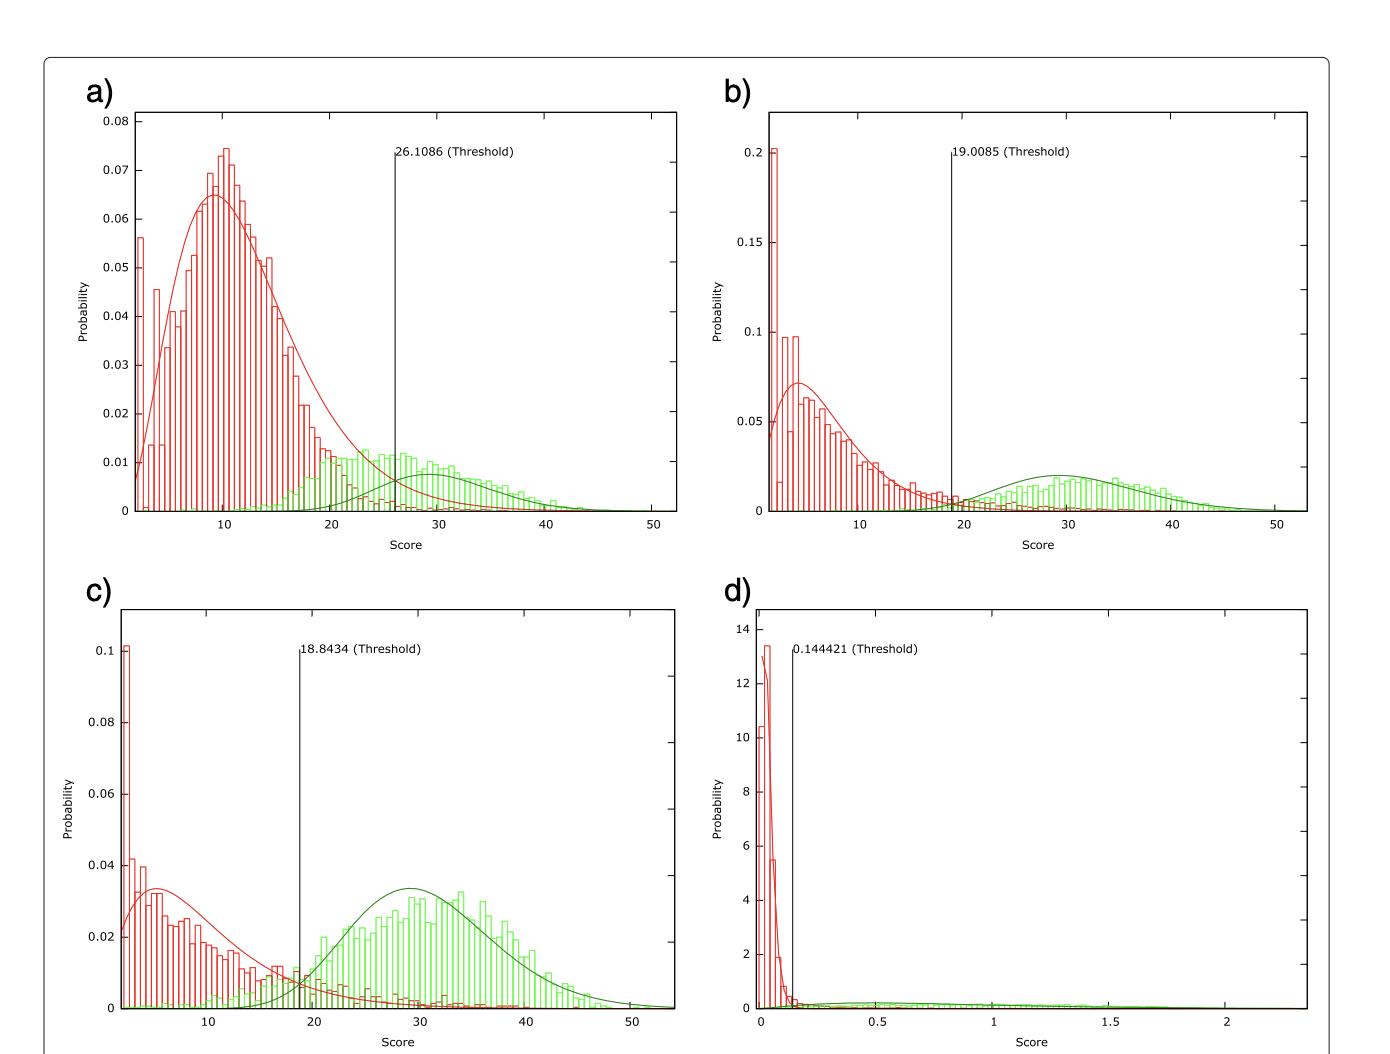
\includegraphics[width=.6\textwidth]{images/mixture_of_two_gammas}
\end{center}
\scriptsize Shown are four gamma mixture models.
\end{sblock}

\vfill \vfill \tiny Landesfeind, M., \& Meinicke, P. (2014). Predicting the functional repertoire of an organism from unassembled RNA–seq data. BMC genomics, 15(1), 1003.

\end{frame}

\begin{frame}{EM for General Mixture Models}
\footnotesize
\begin{sblock}{Algorithm}
\begin{itemize}
\item \bf{E-step:} Recompute the assignment matrix $\soft_{ik}^{(j)}$ as
\[ \soft_{ik}^{(j+1)} = \df{c_k^{(j)}  p(x_i \cond \theta_k^{(j)}) }{ \sum_{l=1}^K c_l^{(j)}  p(x_i \cond \theta_l^{(j)})} \]
\item \bf{M-step:} Recompute $(c,\theta)$ as
\[ (c^{(j+1}, \theta^{(j+1)}) = \arg\max_{c, \theta} \bb{ \ds\sum_{ik} \soft_{ik}^{(j+1)} \log (c_k \, p(x_i \cond \theta_k)) } \]
\end{itemize}
\end{sblock}
\begin{sblock}{Convenient special case}
If the MLE of $p(x \cond \theta)$ is of the form $\widehat{\theta}_{\text{ML}} =\frac{1}{n} \sumn s(x_i)$ for some function $s$  the M-step computes the ``weighted maximum likelihood estimate":
\[ c_k^{(j+1)}  = \df{\sum_{i=1}^n \soft_{ik}^{(j+1)}}{n} \quad \text{and} \quad \theta_k^{(j+1)} = \df{\sumn \soft_{ik}^{(j+1)} s(x_i)}{ \sumn \soft_{ik}^{(j+1)}}\]
This is true for any distribution in the exponential family.\footnote{\tiny Note that the ML problem, and therefore the M-step, need not have closed form solution; e.g. click \blue{\href{https://tminka.github.io/papers/minka-gamma.pdf}{here}} for the Gamma distribution.}
\end{sblock}
\end{frame}



\section{Expectation Maximization (more generally)}

\begin{frame}{Latent variable models}

\begin{itemize}
\item A \textit{parametric statistical model} may posit observed random variables ($\+x$), parameters ($\+\theta$), and latent random variables ($\+z$).   
\item The distinguishing feature between latent variables $\+z$ and parameters $\+\theta$ is that the dimensionality of $\+z$ increases with the size of the data set, whereas the dimensionality of $\+\theta$ does not.\footnote{A more technical definition can be provided via conditional independence.  For example, when there is one latent variable per observation, a latent variable satisfies $p(\+x_n,\+z_n \cond \+x_{-n}, \+z_{-n}, \+\theta) = p(\+x_n,\+z_n \cond \+\theta)$, where the $-n$ subscript refers to the set of variables besides the $n$th. In other words, the $n$th observation and $n$th latent variable is independent of all other observations and latent variables, given the model parameters.}  
\item 
 Note that some presentations refer to $\+z$ as local hidden variables and $\+\theta$ as global hidden variables.
\end{itemize}

\end{frame}

\begin{frame}{Frequentist estimation for latent variable models}
\footnotesize
\begin{itemize}
\item Latent variable models provide a \bf{complete data likelihood}  $p (\+x, \+z \cond \+\theta)$, where $\+z$ is unobserved. The model often factorizes as
\[   p (\+x,  \+z \cond \+\theta) = \ds\prod_{i=1}^n  p (x_i, z_i \cond \+\theta) \]
\item For frequentist latent variable models, the inferential goal is to compute $\+\theta_{\text{ML}}$, the maximum likelihood value of the parameter.  
\item Since $\+z$ is not observed, so one seeks to find 
\begin{equation}
\+\theta_{\text{ML}}:=  \text{argmax}_{\+\theta} \; p (\+x \cond \+\theta) = \text{argmax}_{\+\theta} \ds\int p(\+x,\+z \cond \+\theta) \wrt{\+z} 
\label{ml_latent_vars}
\end{equation}
\item In particular, one requires access to the \textit{marginal} likelihood
\begin{equation}
p(\+x \cond \+\theta) = \ds\int p(\+x,\+z \cond \+\theta) \wrt{\+z} 
\label{marginal_likelihood}
\end{equation}
\end{itemize}
\end{frame}






\begin{frame}{Expectation Maximization for Latent Variable Models}

The \bf{expectation maximization algorithm} estimates $\+\theta$ by attempting to maximize the marginal likelihood. 

The expectation maximization algorithm is 

\begin{equation}
\label{eqn:em_algorithm_appendix}
 \+\theta^{(t+1)} =  \text{argmax}_{\+\theta} \; \E_{p(\+z \cond \+x , \+\theta^{(t)})} \bigg[ \ln p(\+x, \+z \cond \+\theta) \bigg] 
 \end{equation}
\end{frame}

\begin{frame}{Convergence Properties}
\footnotesize
\begin{sblock}{Marginal likelihood}
\begin{itemize}
\item It can be shown that the marginal likelihood $p(\+x \cond \+\theta)$ always increases from each step to the next, unless $\+\theta$ is already a stationary point.
\item The theory guarantees only that the algorithm terminates at a stationary point.  That point can be a saddle point rather than a maximum (very rare)

\end{itemize}
\end{sblock}
\begin{sblock}{The real problem: Local maxima}
\begin{minipage}{.6\textwidth}
\begin{itemize}
\item EM is effectively a gradient method.
\item The maxima it finds are the \bf{local maxima of the log-likelihood}
\item There are no guarantees on the global quality of the solution: The global maximum may differ arbitrarily from the one we find.
\end{itemize}
\end{minipage}
\hfill
\begin{minipage}{.35\textwidth}
\begin{tikzpicture}
  % Put a picture at a tikz node. 
  %I'm not sure what the anchor does, exactly.
    \node[anchor=south west,inner sep=0] (image) at (0,0) {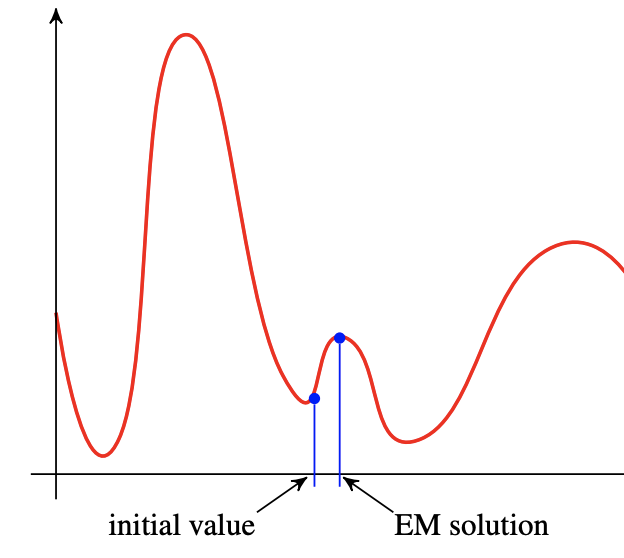
\includegraphics[width=.7\textwidth]{images/em_local_maxima}};
    % The scope environment induces relative coordinates to the picture.
    \begin{scope}[x={(image.south east)},y={(image.north west)}]
        \node[text=black, text width=1cm] at (0,1.2) {$\log p(\+x \cond \+\theta)$};
        \node[text=black, text width=1cm] at (1.2, 0.0) {$\+\theta$};
    \end{scope}
\end{tikzpicture}
\end{minipage}

\end{sblock}
\vfill \tiny \bf{Q:} So what can we do about this?
\end{frame}

\begin{frame}{EM in practice}
\footnotesize
\begin{sblock}{Comparing solutions}
\begin{itemize}
\item If $\+\theta$ and $\+\theta^\prime$ are two different EM solutions, we can always compute the log-likelihoods
\[ \ds\sum_i \log p(x_i \cond \+\theta) \quad \text{and} \quad \ds\sum_i \log p(x_i \cond \+\theta^\prime) \]
\item The solution with the higher likelihood is better.
\item This is a very convenient feature of EM: Different solutions are comparable. 
\end{itemize}
\end{sblock}
\begin{sblock}{Random restarts}
In practice, the best way to use EM is often
\begin{itemize}
\item Restart EM repeatedly with randomly (or intelligently) chosen initial values.
\item Compute the log-likelihoods of all solutions and compare them.
\item Choose the solution achieving maximal log-likelihood
\end{itemize}
\end{sblock}
\vfill
\tiny \bf{Q}: What would be an intelligent way to initialize?
\end{frame}


\begin{frame}{EM for Exponential Family Latent Variable Models}
\scriptsize 
%We see how this plays out in the exponential family.   
Let us assume that $(\+x, \+z)=((x_1,z_1), ..., (x_n, z_n))$ are $n$ independent samples from the same exponential family, where $\+x$ is observed data and $\+z$ is unobserved data.
Moreover, let us assume that the complete data likelihood is in the exponential family

\begin{align}
\label{eqn:exponential_family_complete_data_likelihood}
 p(\+x, \+z \cond \theta) = \ds\prod_{i=1}^n h(x_i, z_i) \exp \big\{ \eta(\theta)^T \sum_{i=1}^n t(x_i, z_i) - n \,a(\eta(\theta))\big\} 
 \end{align}

Here we want to find $\+\theta$ to optimize 
\[ f(\+\theta) =  \E_{p(\+z \cond \+x , \+\theta^{(t)})} \bigg[ \ln p(\+x, \+z \cond \+\theta) \bigg] \]

Following the logic of the Exponential Family module, we determine that we should select $\theta^{(t+1)}$ such that
\[ \mu(\theta^{(t+1)}) = \df{1}{n} \ds\sum_{i=1}^n   \E_{p(\+z \cond \+x , \+\theta^{(t)})} t(x_i, z_i) \]
where $\mu := \E[t(x_1,z_1)]$ refers to the mean parametrization of the likelihood.

This is why an EM iteration is often described and  implemented as iteratively computing \bf{maximum likelihood with the expected sufficient statistics.}
\end{frame}

\section{Some Cybersecurity Applications of EM}
\subsection{Better malware ground truth}
\begin{frame}{Introduction}
\begin{itemize}
\item Commercial anti-virus software traditionally memorizes specific byte sequences (known as \textbf{signatures}) in the file contents of previously encountered malware. 
\item They could use these signatures to attempt to detect malware in the future.
\item Malware authors can evade signature-based detection in many ways; for instance, by
	\begin{itemize}
	\item tampering with existing malware signatures (sometimes flipping a single bit)
	\item  using obfuscation techniques (e.g. encryption or compression) to hide snippets of malicious code
	\item writing metamorphic malware
	\end{itemize}
\item As a result, classical AV detections have \bf{low false positive} rates \it{but also} \bf{low true positive} rates.
\end{itemize}
\end{frame}

\begin{frame}{Better Malware Ground Truth}
Kantchelian et al. (2015) examine the problem of aggregating the results of multiple anti-virus (AV) vendors’ detectors into a single authoritative ground-truth label for every binary
\vfill \vfill \vfill
\tiny Kantchelian, A., Tschantz, M. C., Afroz, S., Miller, B., Shankar, V., Bachwani, R., ... \& Tygar, J. D. (2015, October). Better malware ground truth: Techniques for weighting anti-virus vendor labels. In Proceedings of the 8th ACM Workshop on Artificial Intelligence and Security (pp. 45-56).
\end{frame}

\begin{frame}{Model}
\footnotesize
\begin{sblock}{Random variables}

\begin{minipage}{.6\textwidth}
\begin{align*}
X_{ij} & \in \set{0,1} && \text{ AV label (i = instance, j =vendor)} \\
Z_i & \in \set{0,1} && \text{ground truth label} \\
\alpha, \beta & && \text{vendor tp, fp rates} \\
\pi & && \text{malware prevalence} 
\end{align*}

In our terminology, $\+Z$ are latent variables and $\alpha, \beta$ are parameters.
\end{minipage}
\hfill
\begin{minipage}{.35\textwidth}
\begin{center}
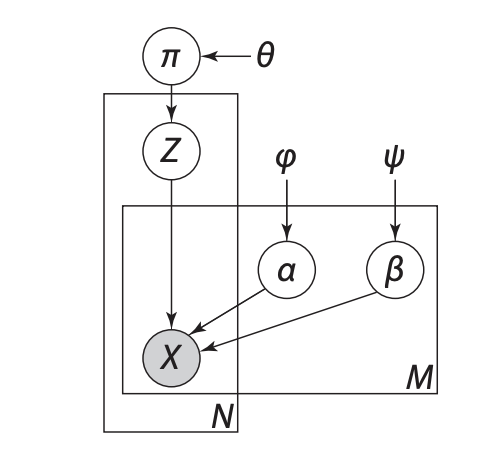
\includegraphics[width=.7\textwidth]{images/kantchelian_pgm}
\end{center}
\end{minipage}


\end{sblock}

\begin{sblock}{Model}

\begin{minipage}{.65\textwidth}
\begin{align*}
X_{ij} \cond Z_{i}, \alpha_j, \beta_j &= 
\begin{cases}
\alpha_j&  \text{ if } Z_i  =1   \text{ and }  X_{ij} = 1  \;  \text{(TP)} \\
1 - \alpha_j&  \text{ if }  Z_i  =1    \text{ and } X_{ij} = 0     \; \text{(FN)} \\
\beta_j &  \text{ if }  Z_i  =0  \text{ and } X_{ij} = 1     \; \text{(FP)} \\
1 - \beta_j& \text{ if } Z_i  =0  \text{ and } X_{ij} = 0    \;  \text{(TN)} \\
\end{cases} \\
Z_i \cond \pi & \sim \text{Bernouli}(\pi) \\
\pi &\sim \text{Beta (symmetric)} \\
\alpha \cond \psi &\sim \text{Beta (assymmetric)} \\
\beta \cond \phi &\sim \text{Beta (assymmetric)} \\
\end{align*}
\end{minipage}
\hfill 
\begin{minipage}{.3\textwidth}
\begin{center}
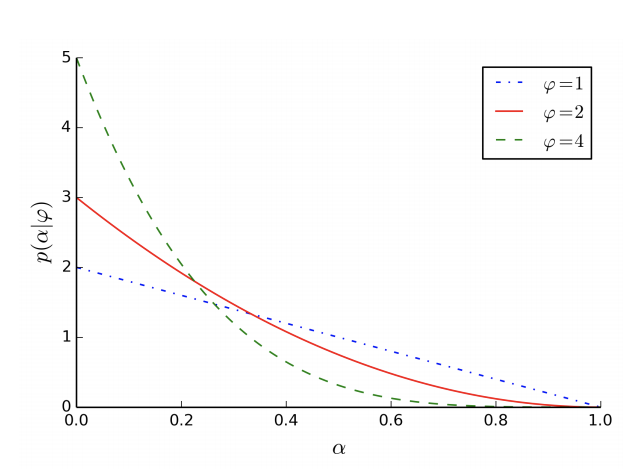
\includegraphics[width=\textwidth]{images/assymmetric_beta_kantchelian}

\scriptsize Asymmetric (right skewed) priors were used for $\alpha, \beta$ since both are expected to be low based on prior domain knowledge. 
\end{center}

\end{minipage}

\end{sblock}

\vfill \vfill \vfill \bf{Rk:} This is actually a \textit{Bayesian} latent variable model, since the parameters are assumed to be random variables.  However, we do not focus on that point here.
\end{frame}

\begin{frame}{Estimation and Results}

\begin{itemize}
\item The model was fit using EM.
\item The model far outperforms a common baseline in estimating ground truth.
\begin{center}
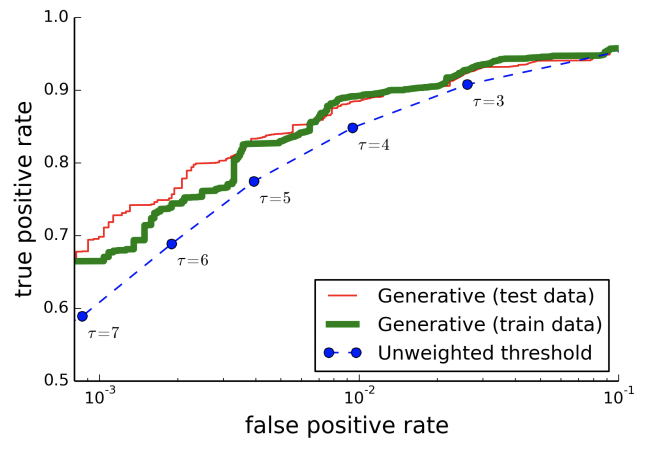
\includegraphics[width=.6\textwidth]{images/kantchelian_performance}
\end{center}
\item Moreover, it accomplished this \it{despite being fully unsupervised}!  (No ground truth was available during training.)
\end{itemize}

\end{frame}

\subsection{Behavioral biometrics}
\begin{frame}{Keystrokes biometrics}

Gaussian mixture models (and other density models) have been applied to typing behavior to flag anomalous behavior.

\begin{center}
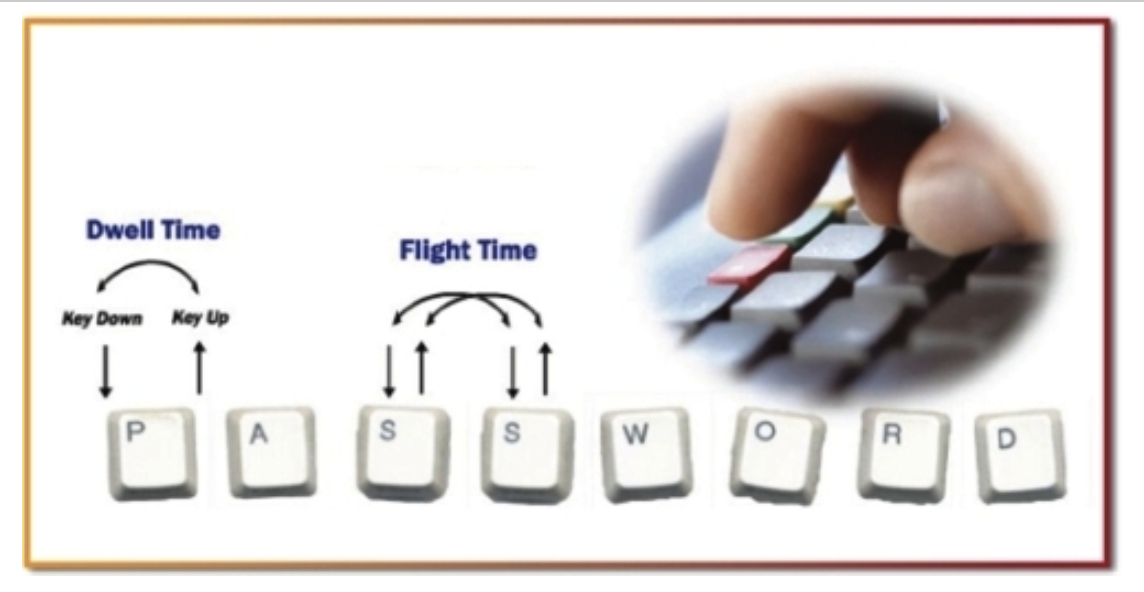
\includegraphics[width=\textwidth]{images/keystroke_dynamics}
\end{center}

\end{frame}

\end{document}




%THE ACTUAL KANTCHELIAN MODEL.
\begin{sblock}{Model}

\begin{minipage}{.65\textwidth}
\begin{align*}
X_{ij} \cond Z_{i}, \alpha_j, \beta_j &= 
\begin{cases}
\alpha_j&  \text{ if } Z_i  =1   \text{ and }  X_{ij} = 1  \;  \text{(TP)} \\
1 - \alpha_j&  \text{ if }  Z_i  =1    \text{ and } X_{ij} = 0     \; \text{(FN)} \\
\beta_j &  \text{ if }  Z_i  =0  \text{ and } X_{ij} = 1     \; \text{(FP)} \\
1 - \beta_j& \text{ if } Z_i  =0  \text{ and } X_{ij} = 0    \;  \text{(TN)} \\
\end{cases} \\
Z_i & \sim \text{Bernouli}(\pi) \\
\pi &\sim \text{Beta (symmetric)} \\
\alpha \cond \psi &\sim \text{Beta (assymmetric)} \\
\beta \cond \phi &\sim \text{Beta (assymmetric)} \\
\end{align*}
\end{minipage}
\hfill 
\begin{minipage}{.3\textwidth}
\begin{center}
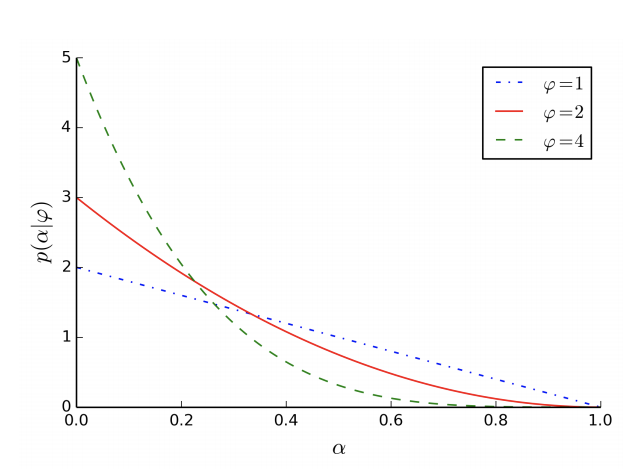
\includegraphics[width=\textwidth]{images/assymmetric_beta_kantchelian}
Assymmetric Beta (right skewed) were used since 
\end{center}

\end{minipage}

\end{sblock}

\vfill \vfill \vfill \bf{Rk:} This is actually a \textit{Bayesian} latent variable model, since the parameters are assumed to be random variables.  However, we do not focus on that point here.
\end{frame}




\begin{frame}{Hyperparameters}
\begin{tikzpicture}
  % Put a picture at a tikz node. 
  %I'm not sure what the anchor does, exactly.
    \node[anchor=south west,inner sep=0] (image) at (0,0) {\includegraphics[width=\textwidth]{images/bd_ihmm_hyperparameters}};
    % The scope environment induces relative coordinates to the picture.
    \begin{scope}[x={(image.south east)},y={(image.north west)}]
        \node[text=blue, text width=2cm] at (.30, 1.2) {more states};
        \node[text=blue, text width=2cm] at (.50, 1.2) {more blocks};
         \node[text=blue, text width=2cm] at (.70, 1.2) {freer mvmt across blocks};
        \node[text=blue, text width=2cm] at (.90, 1.2) {$\downarrow$ variability in transition probabilities};
    \end{scope}
\end{tikzpicture}
\scriptsize Truncated Markov transition matrices (right stochastic) sampled from the BD-iHMM prior with various fixed hyperparameter values.  Highlighted hyperparameters yield the chief observable difference from the leftmost matrix.
\end{frame}

